\begin{frame}{}

\section{Ionisation Modelling}

\vspace*{1cm}

{\huge{\textbf{Ionisation Modelling}}}

\end{frame}



\begin{frame}{\huge{{\textbf{Method}}}}

\uncover<1->{\begin{itemize}

    \item<2-> \only<2>{\textbf{Grid of PI CLOUDY models : Density and Metallicity}} \only<3->{Grid of PI CLOUDY models : Density and Metallicity} 
    \item<3-> \only<3>{\textbf{log (${\text{n}}_{\text{H}} / \text{cm}^{-3}$)} : -5 to 1 in steps of 0.02} \only<4->{log (${\text{n}}_{\text{H}} / \text{cm}^{-3}$) : -5 to 1 in steps of 0.02} 
    \item<4-> \only<4>{\textbf{log ($\text{Z/Z}\odot$)} : -3 to 2 in steps of 0.05} \only<5->{log (Z/$Z\odot$) : -3 to 2 in steps of 0.04}  
    \item<5-> \only<5>{\textbf{Solution : Model that best predicts the observed column densities}}

\end{itemize}
}

\begin{tikzpicture}[remember picture, overlay,use page relative coordinates]
    
    \uncover<2->{\node at (0.25,0.15) {\footnotesize{Ref. : Acharya and Khaire (2021)}} ;} 
    
\end{tikzpicture}

\end{frame}



\begin{frame}{\huge{{\textbf{Results}}}}

\uncover<1->{\begin{itemize}
    
    \item<2-> \only<2>{\textbf{17 \ion{O}{vi} absorbers : 25 components}} \only<3->{17 \ion{O}{vi} absorbers : 25 components}
    \item<3-> \only<3>{\textbf{12 non-\ion{O}{vi} absorbers : 14 components}} \only<4->{12 non-\ion{O}{vi} absorbers : 14 components}
    \item<4-> \only<4>{\textbf{Origin of \ion{O}{vi}}}
    
\end{itemize}
}

\end{frame}


\begin{frame}[noframenumbering]{\textbf{Solutions}}

\begin{figure}[!htbp]
    \centering
    \vspace*{-2mm}
    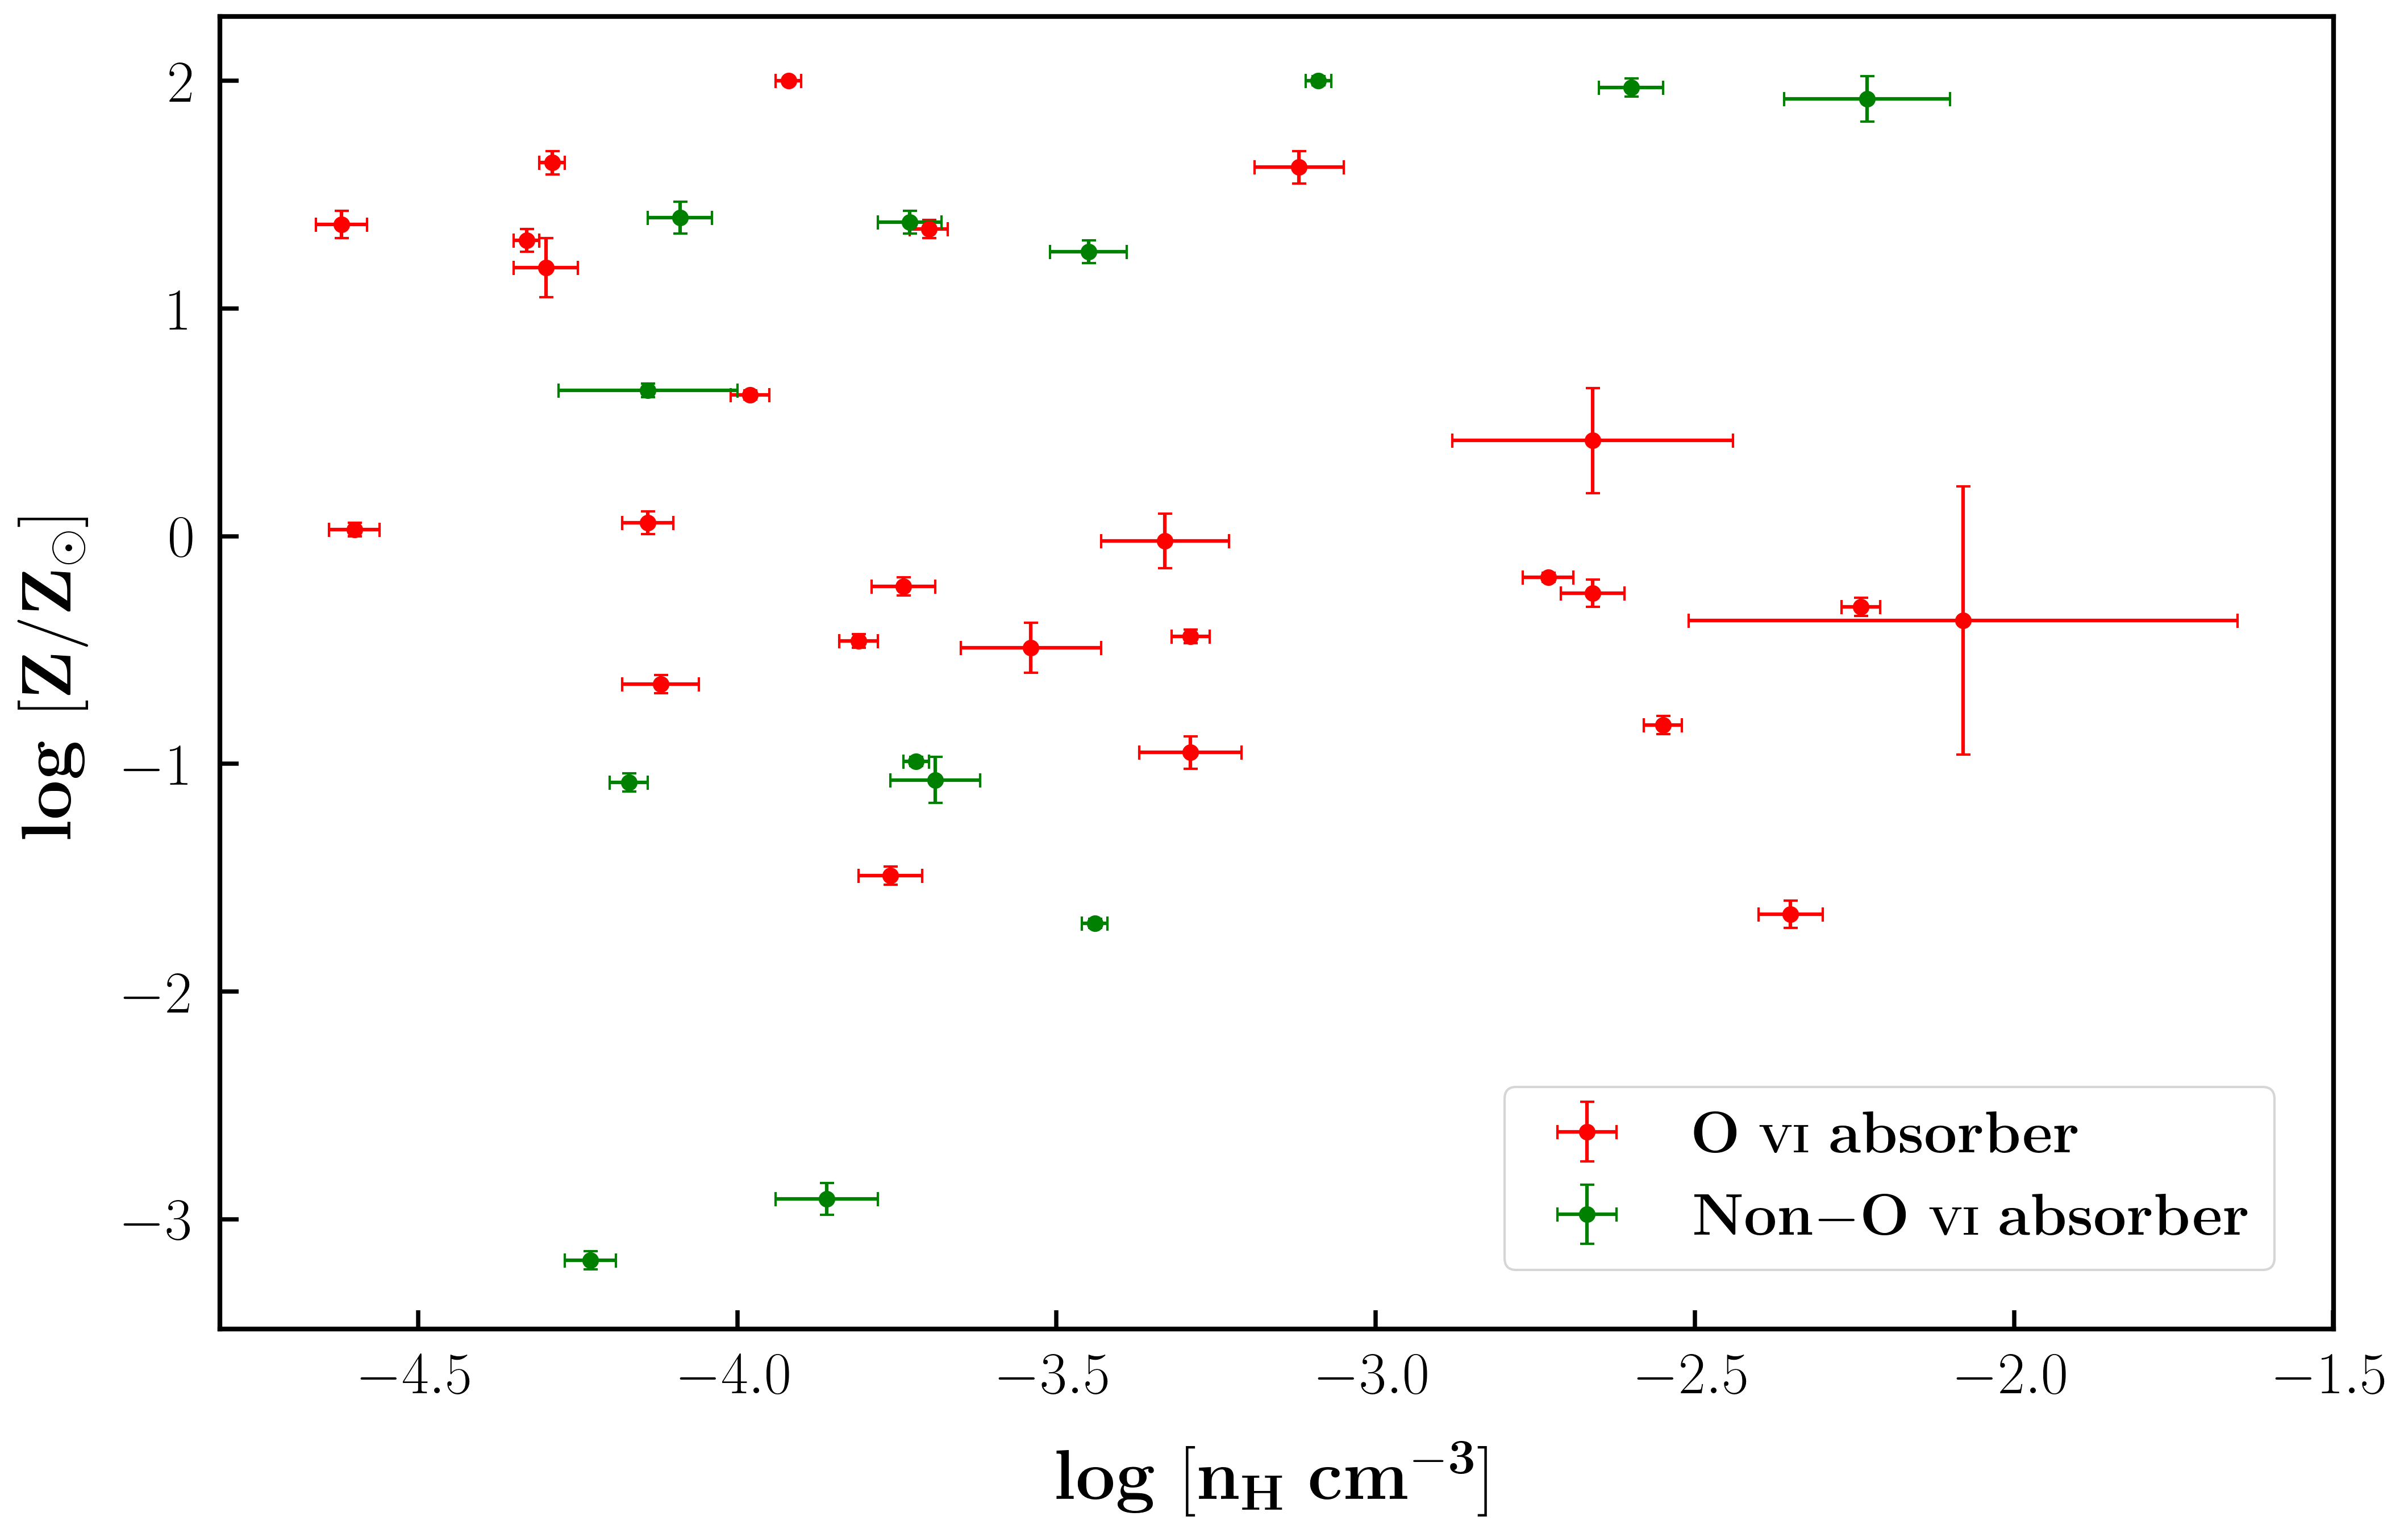
\includegraphics[width=10cm]{Figures-Thesis/Z_vs_nH.png}
    \vspace*{-1mm}
    \caption{Ionisation modelling solutions ($\text{n}_\text{H}, Z$) for all 39 components.}
\end{figure} 


\end{frame}


\begin{frame}[noframenumbering]{\textbf{+ve correlation}}

\begin{figure}[!htbp]
    \centering
    \vspace*{-2mm}
    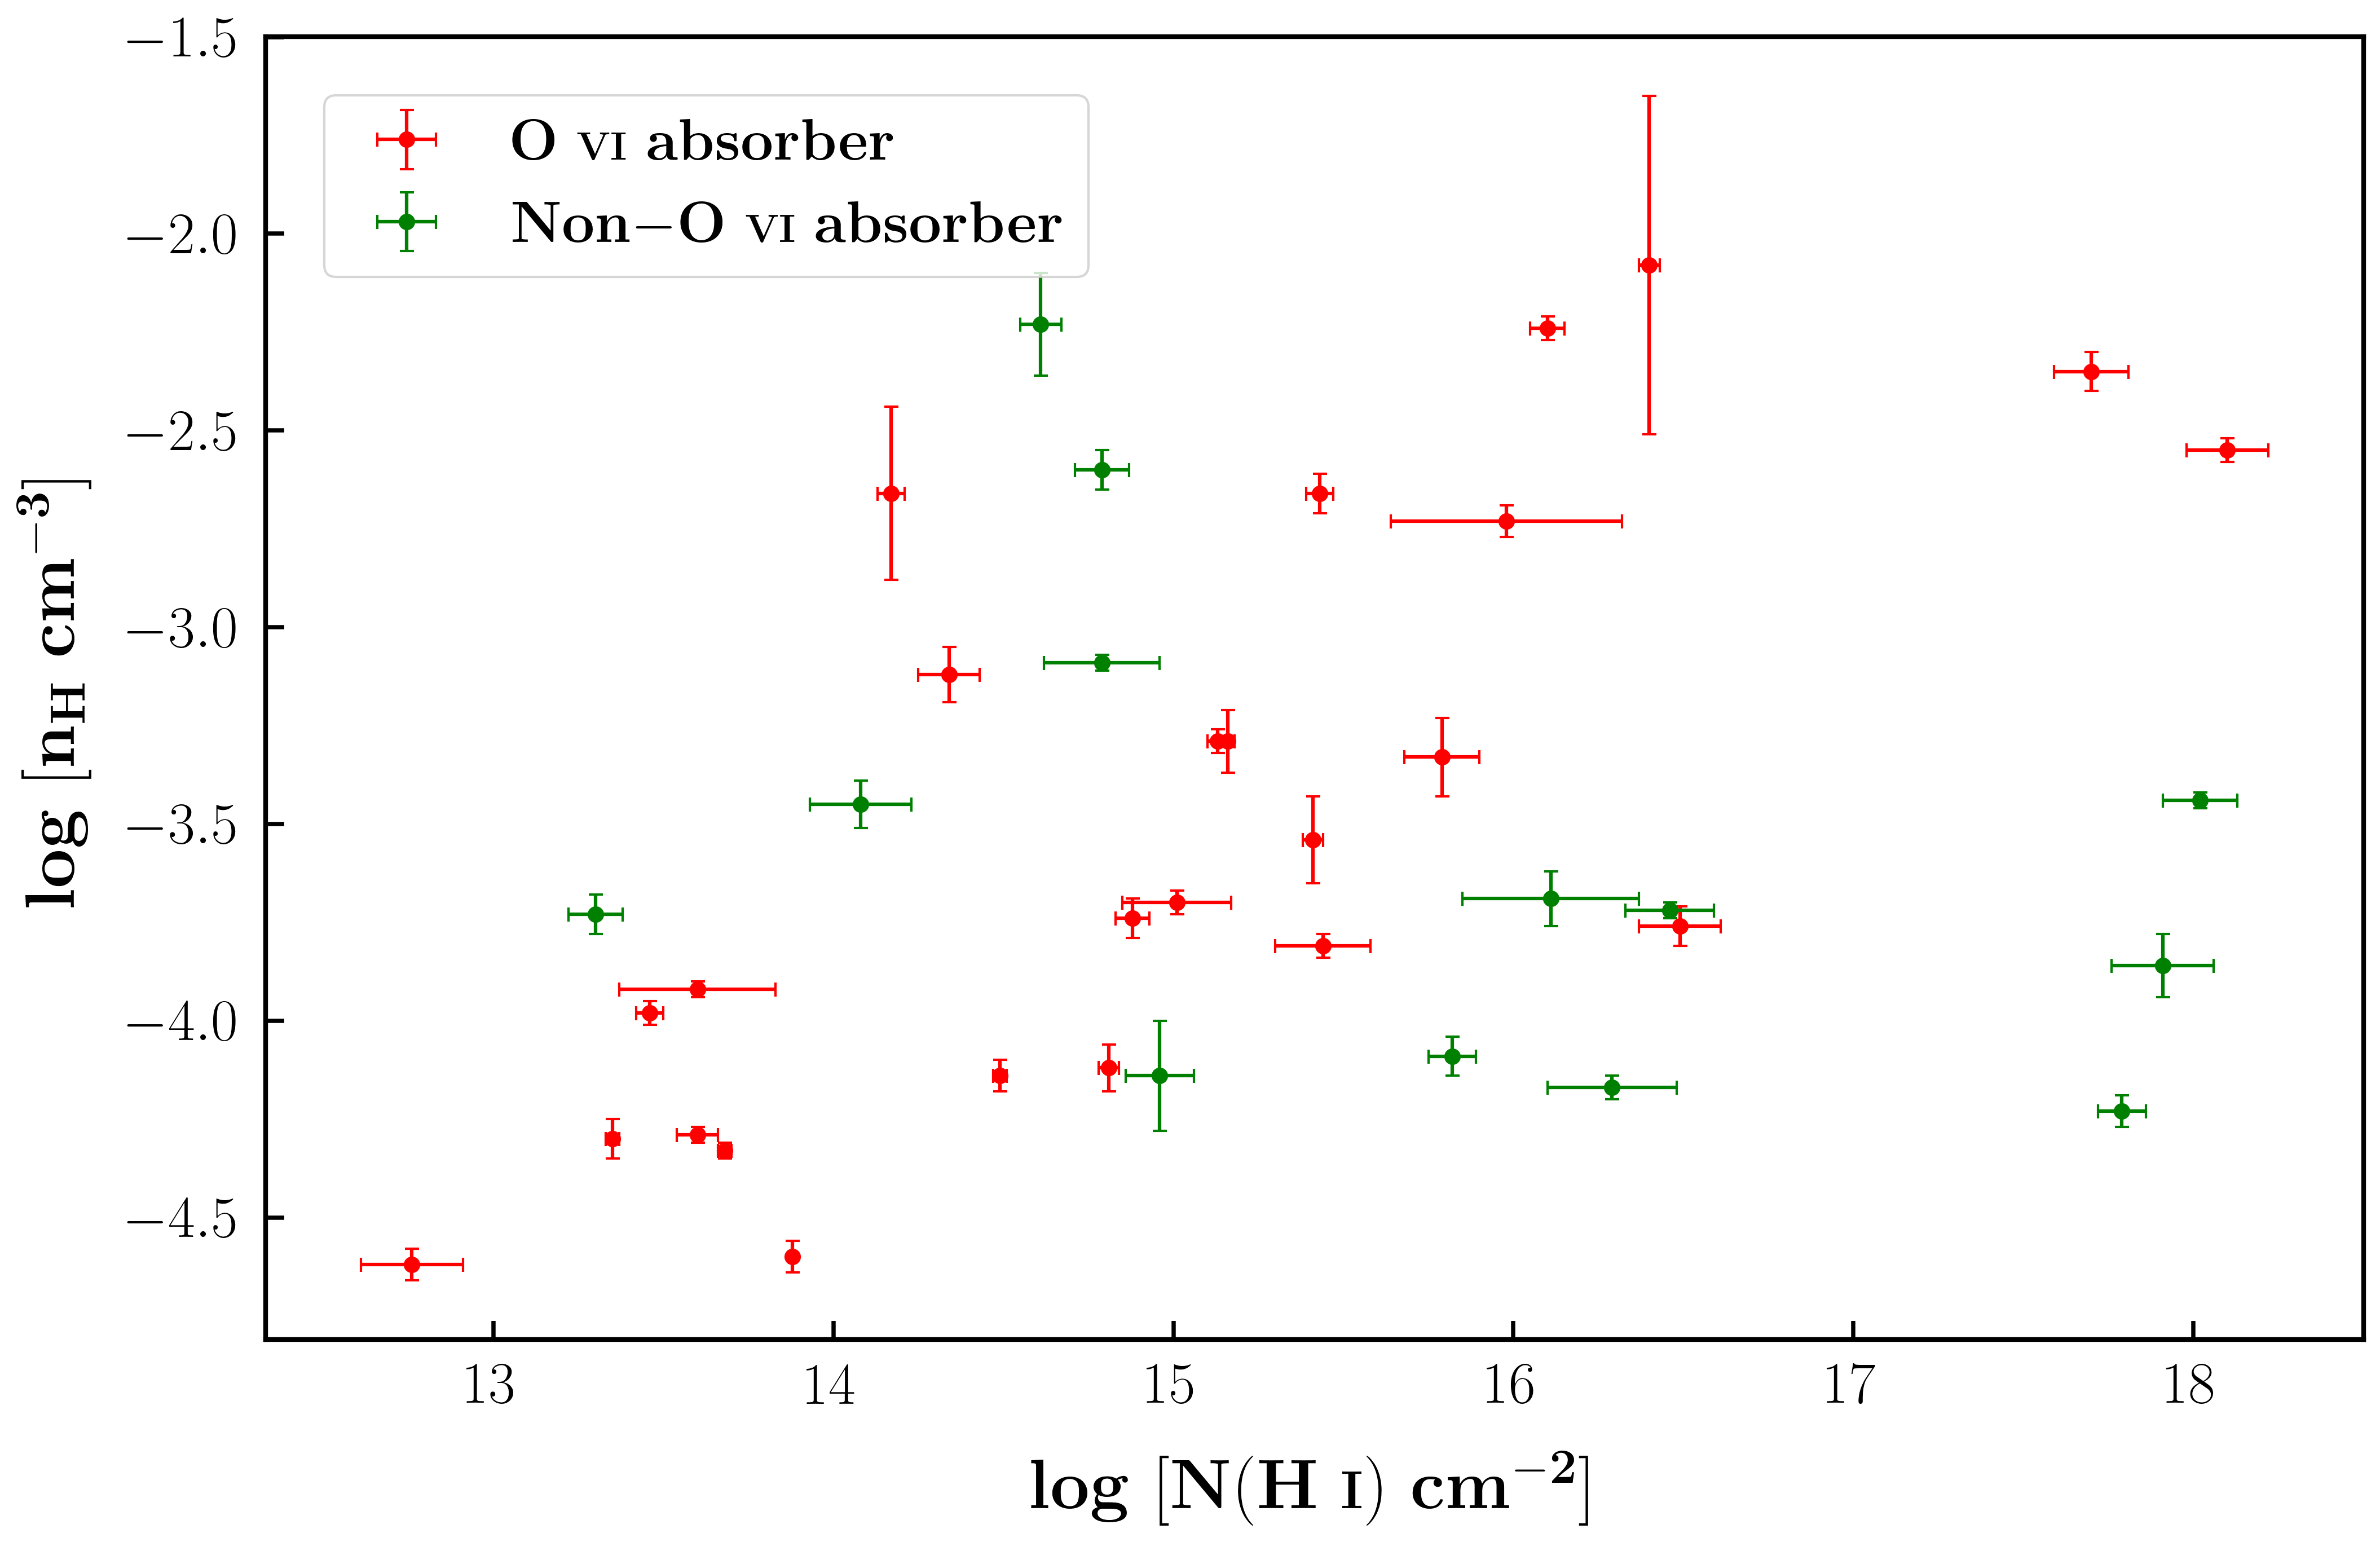
\includegraphics[width=10cm]{Figures-Thesis/nH_vs_NHi.png}
    \vspace*{-1mm}
    \caption{Variation of $\text{n}_\text{H}$with N(\ion{H}{i})}
\end{figure}  

\end{frame}


\begin{frame}[noframenumbering]{\textbf{-ve correlation}}

    \begin{figure}[!htbp]
    \centering
    \vspace*{-2mm}
    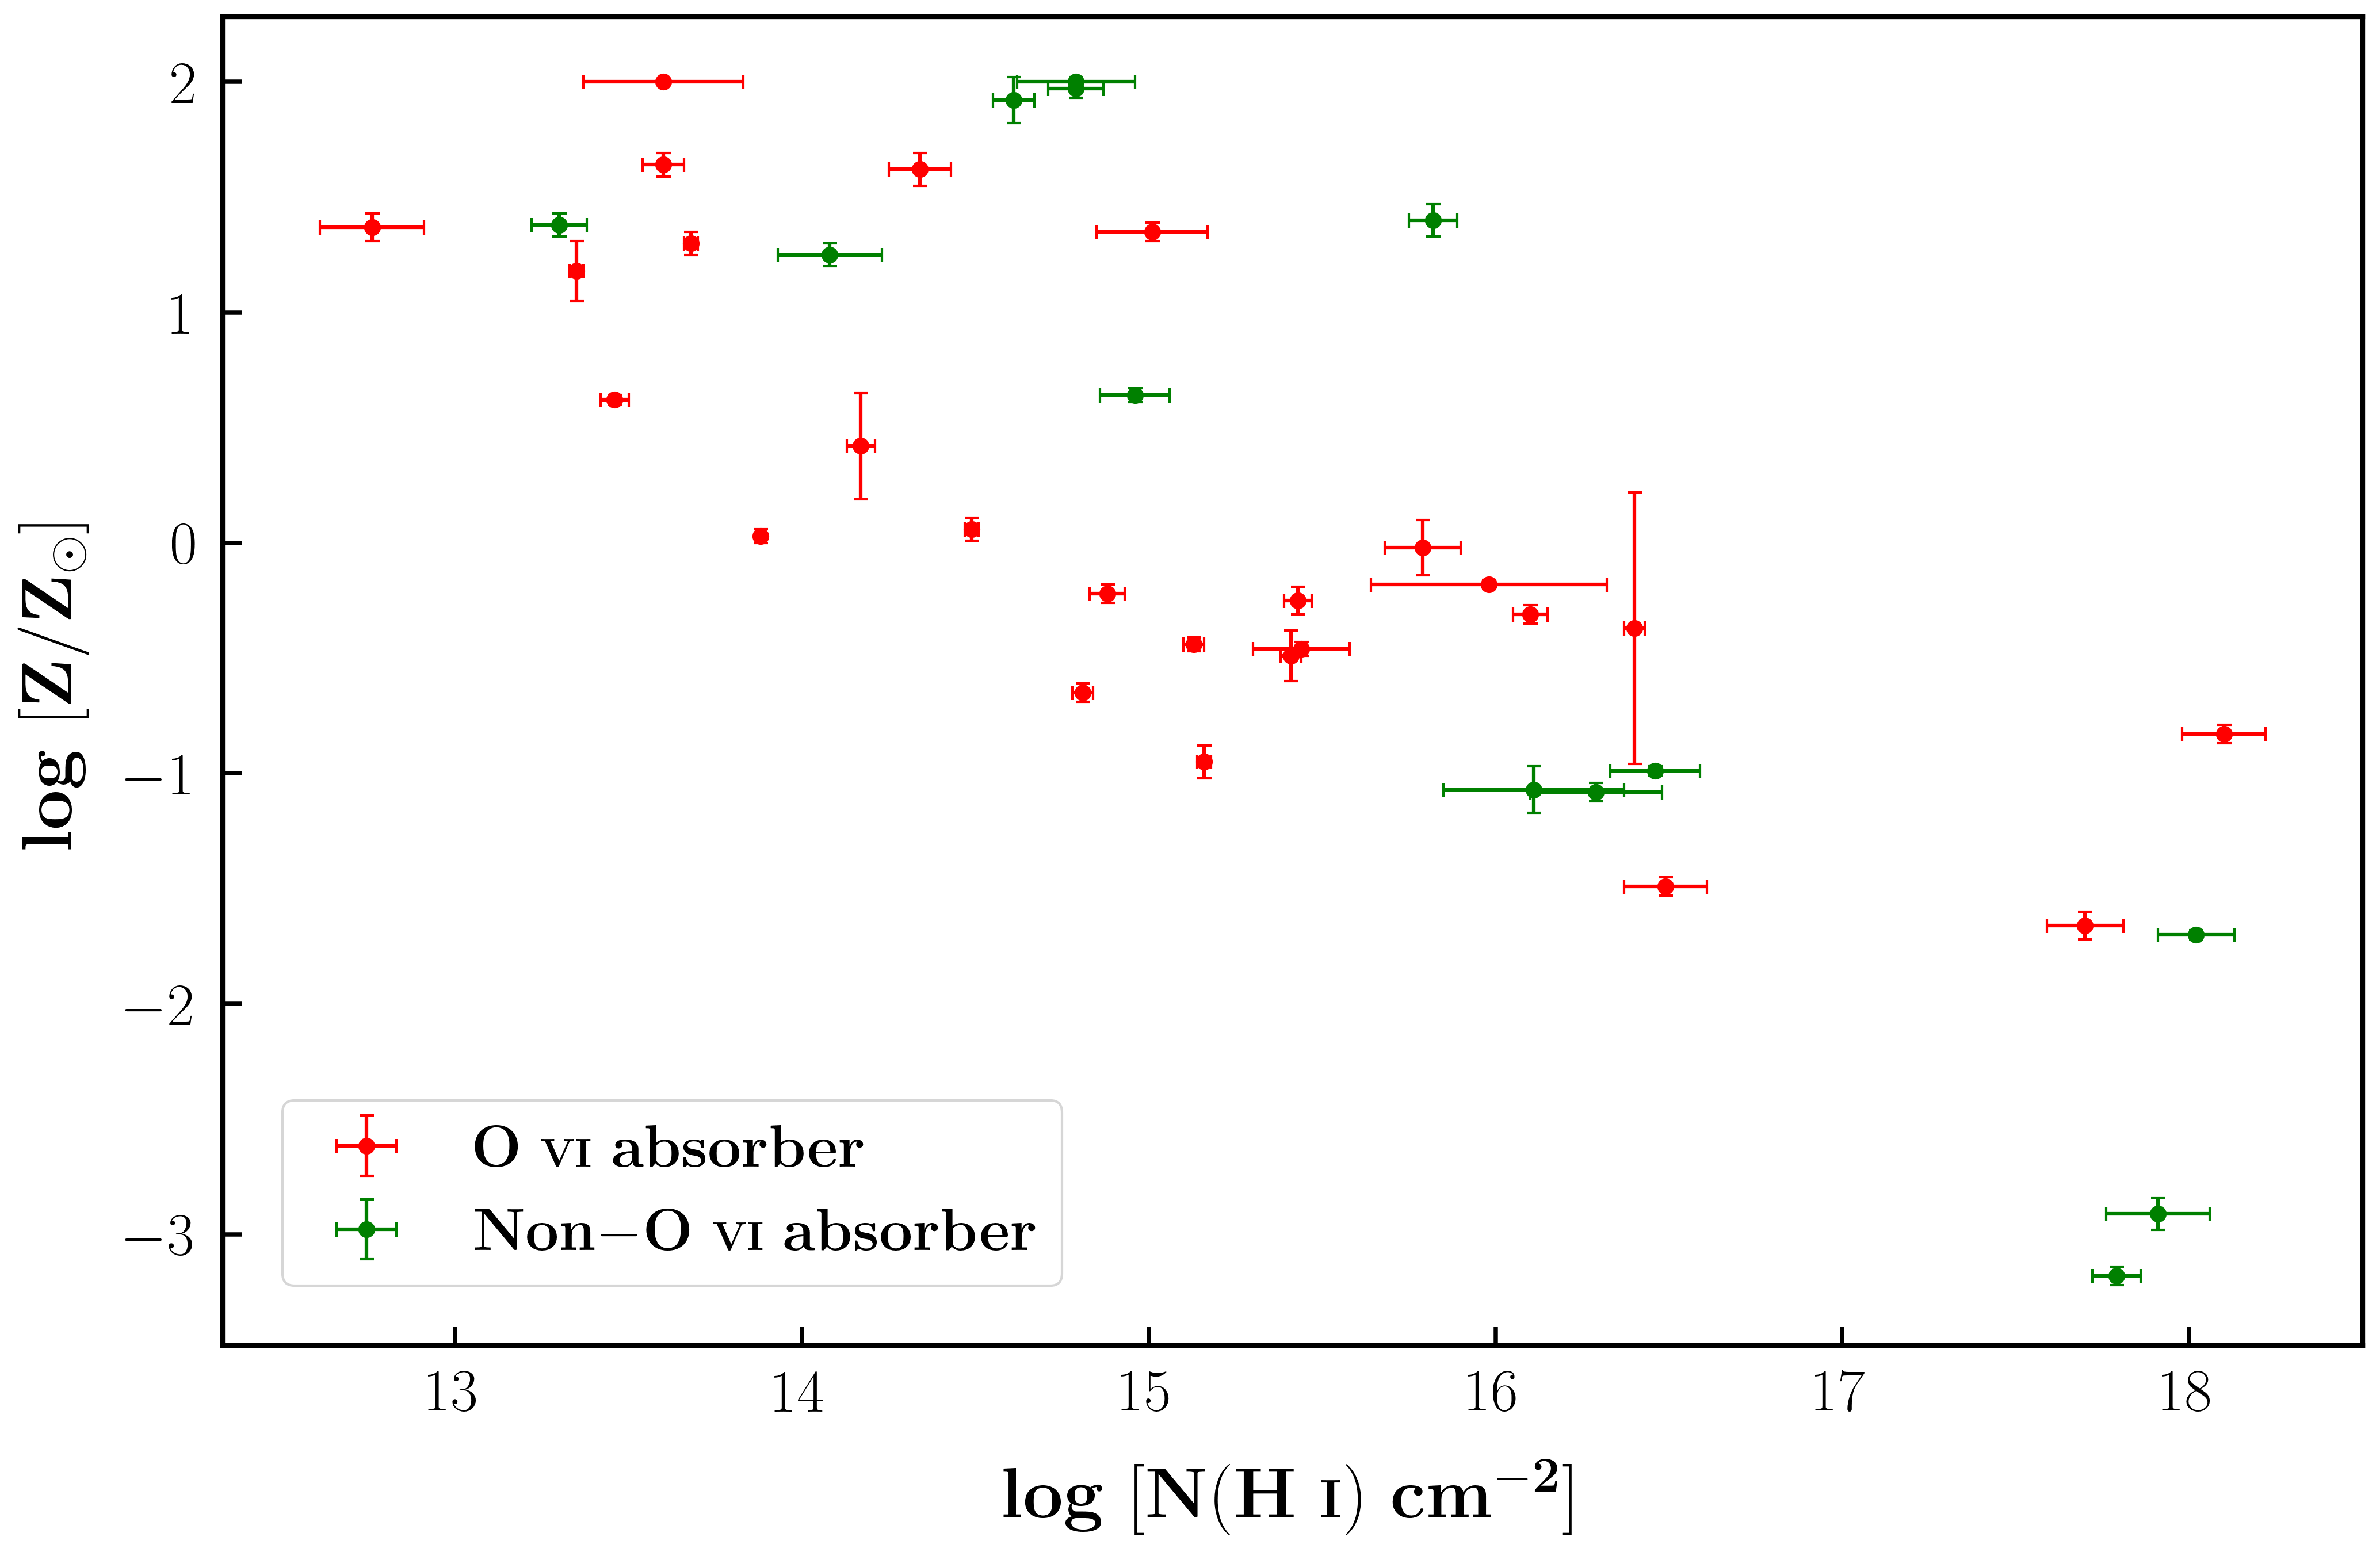
\includegraphics[width=10cm,draft=False]{Figures-Thesis/Z_vs_NHi.png}
    \vspace*{-1mm}
    \caption{Variation of $Z$ with N(\ion{H}{i})}
    \end{figure}  
    
    \end{frame}


\begin{frame}{\textbf{Origin of \ion{O}{vi}}}

\begin{figure}[!htbp]
    \centering
    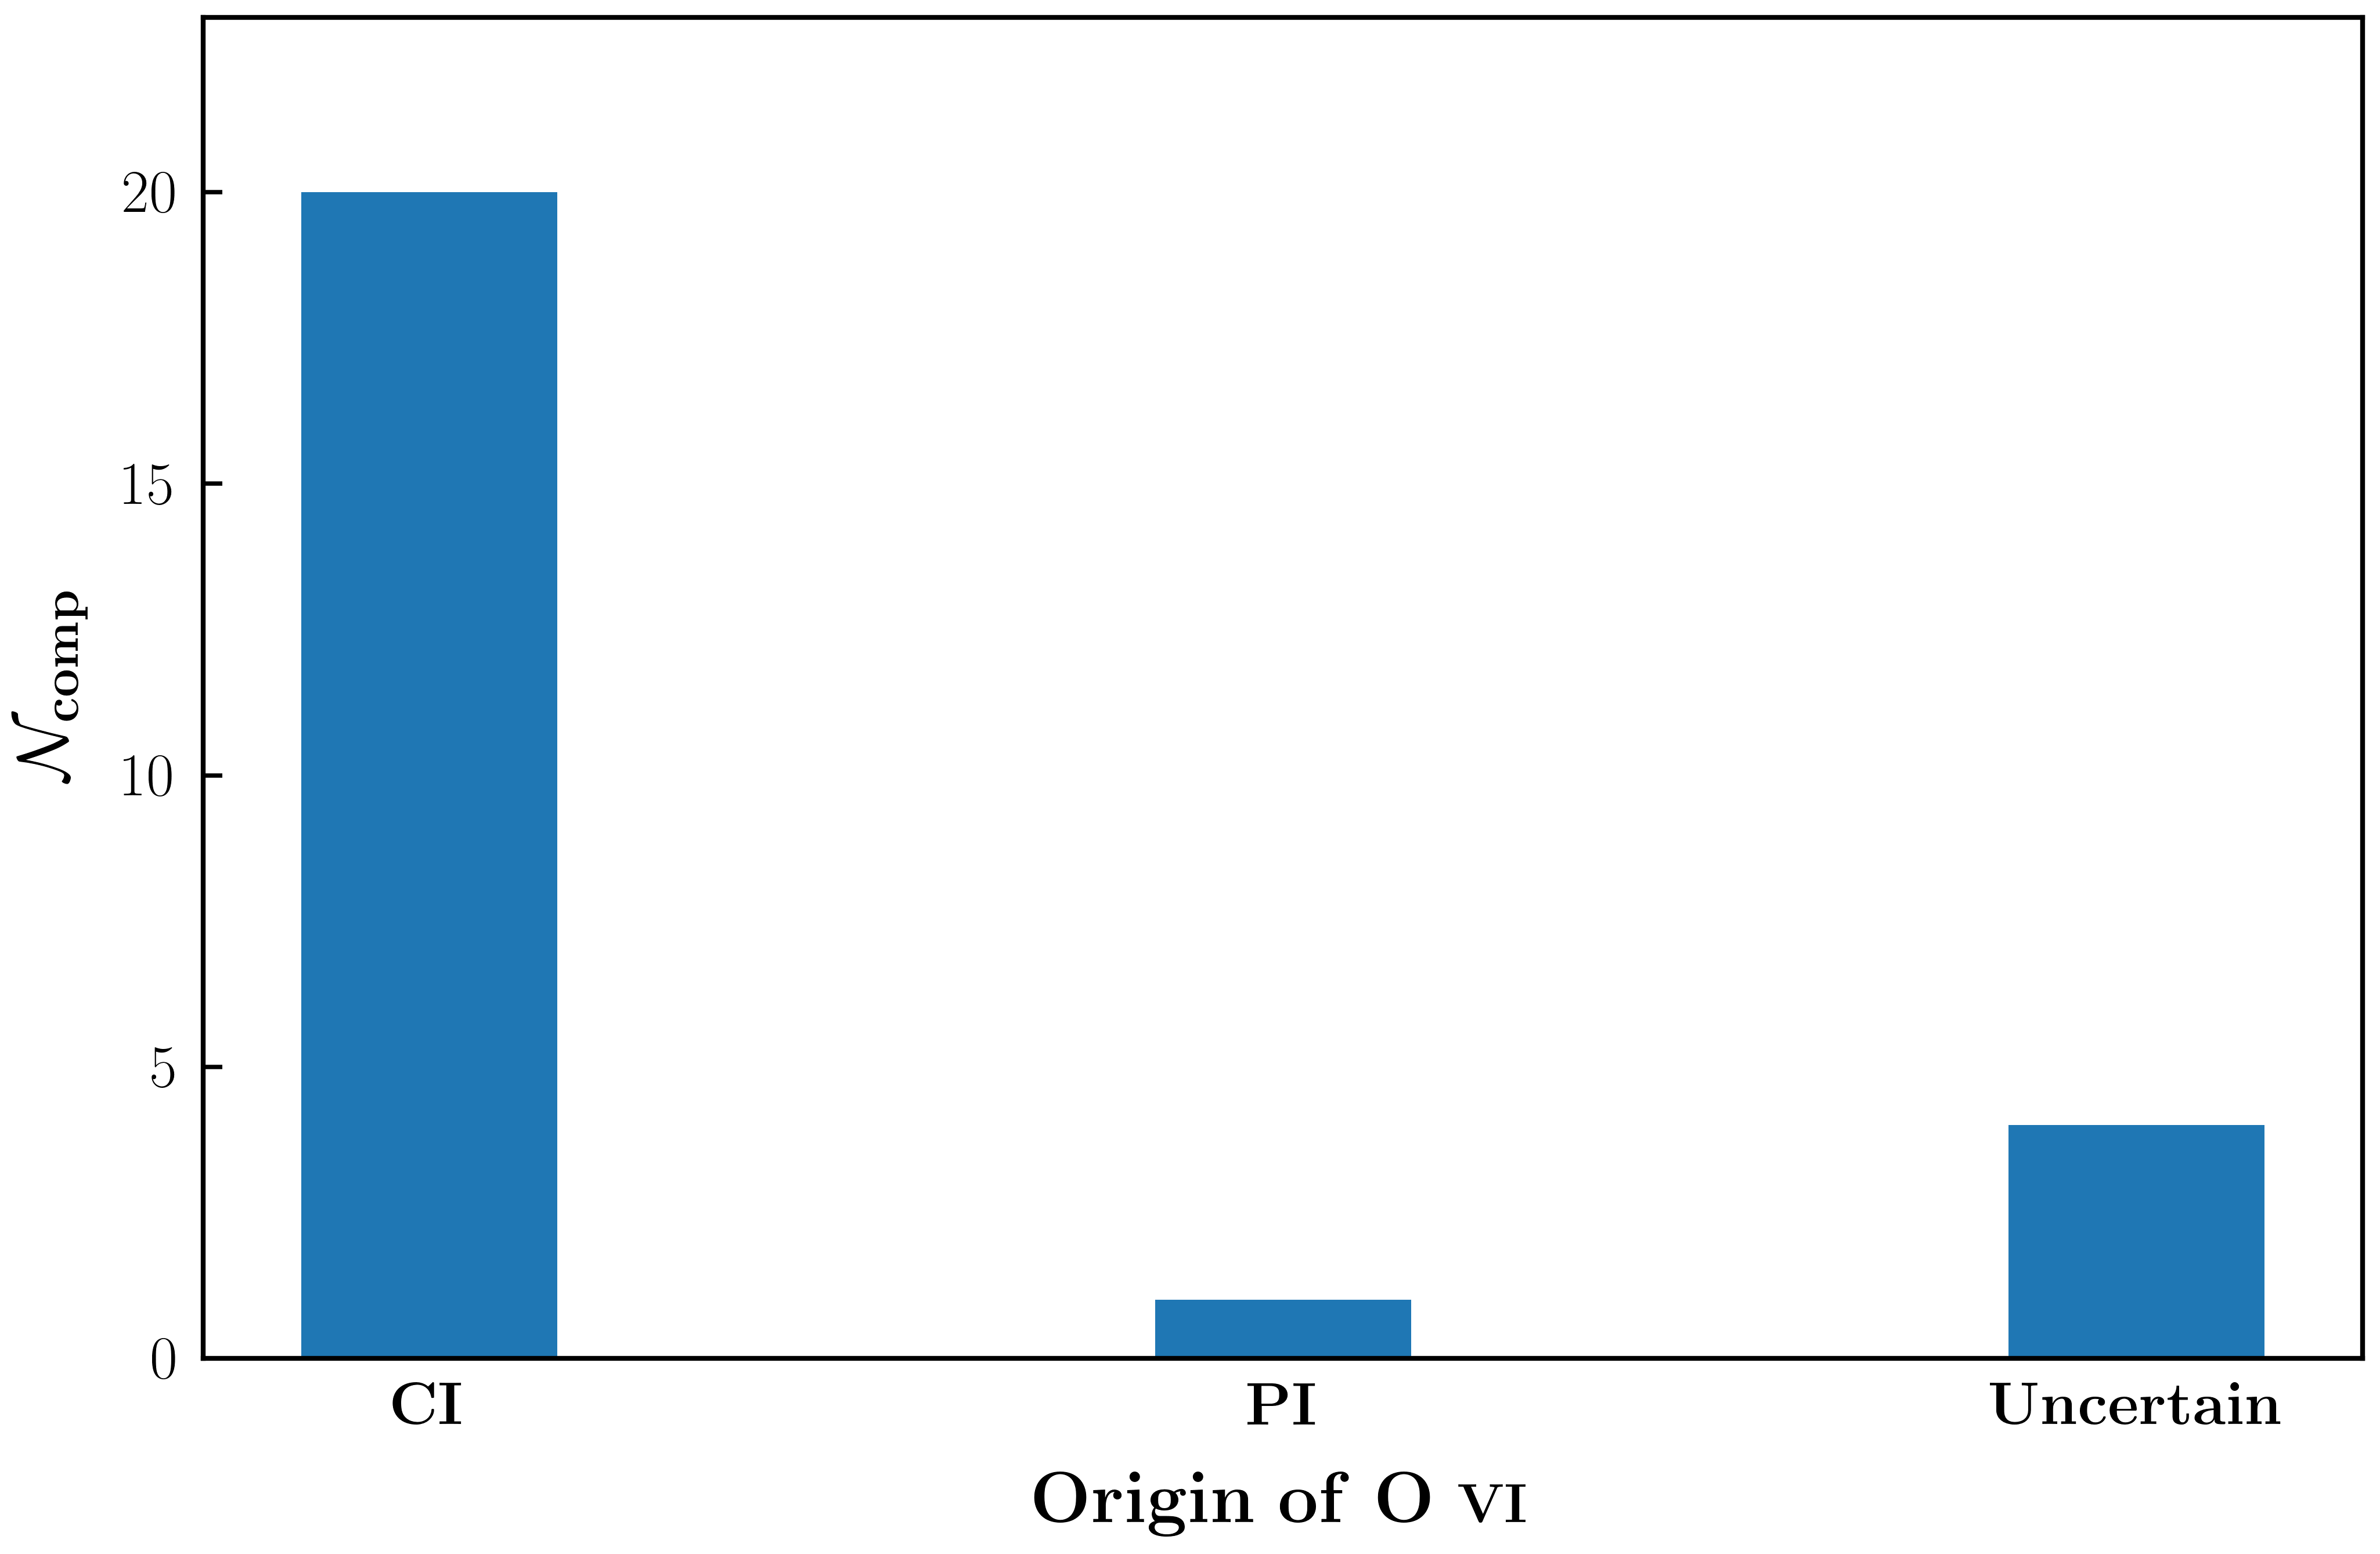
\includegraphics[width=9cm]{Figures-Thesis/OVI_cases.png}
    \vspace*{-1mm}
    \caption{Ionisation state of \ion{O}{vi} inferred from ionisation modelling}
\end{figure}  

\end{frame}



\begin{frame}[noframenumbering]{\textbf{Ex : CI}}

\begin{figure}[!htbp]
    \centering
    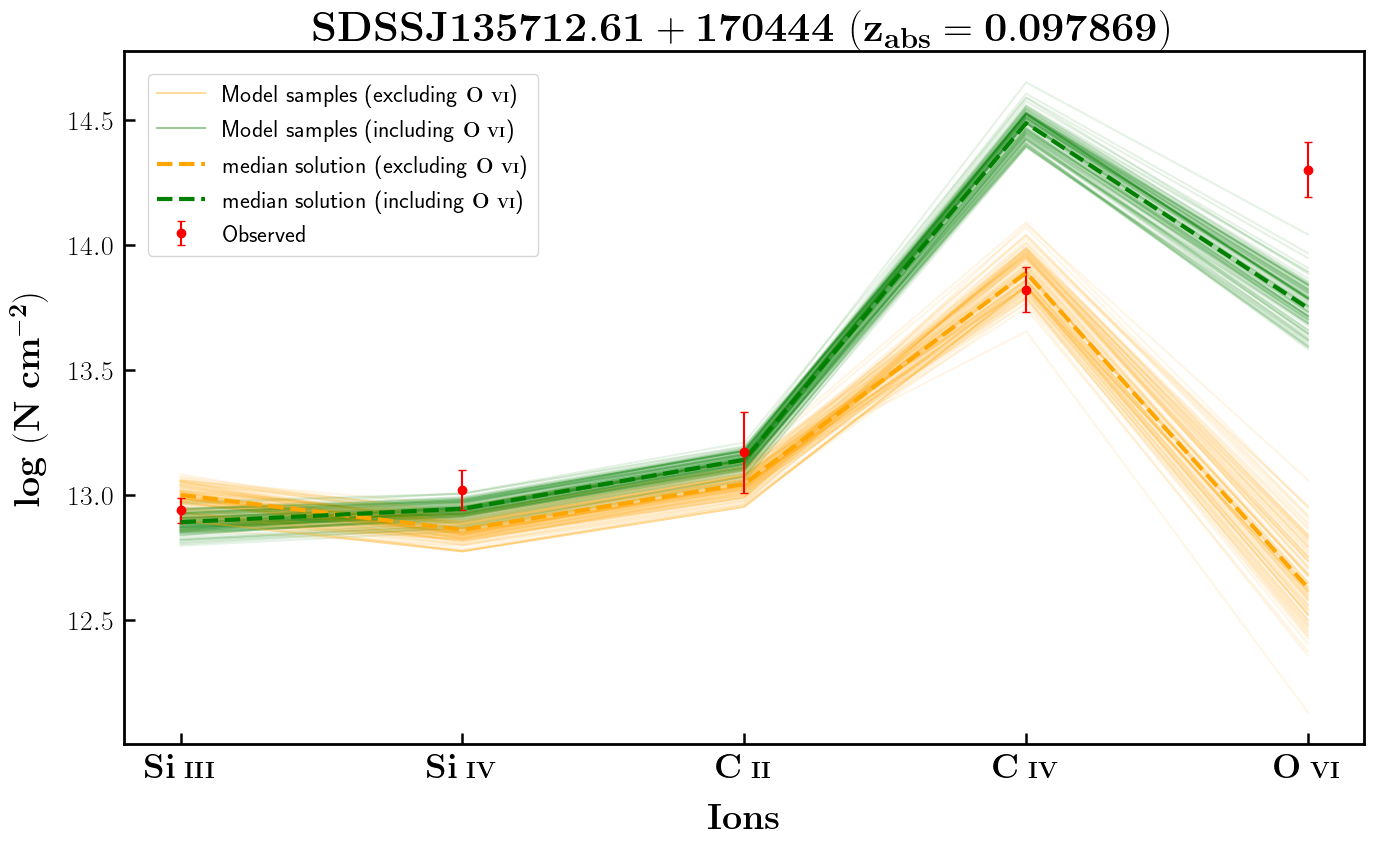
\includegraphics[width=10cm]{Figures/s135712-z=0.097869-compII.png}
    \vspace*{-1mm}
    \caption{log N(\ion{H}{i}) [cm$^{-2}$]=16.49}
\end{figure}  

\end{frame}


\begin{frame}[noframenumbering]{\textbf{Ex : PI}}

\begin{figure}[!htbp]
    \centering
    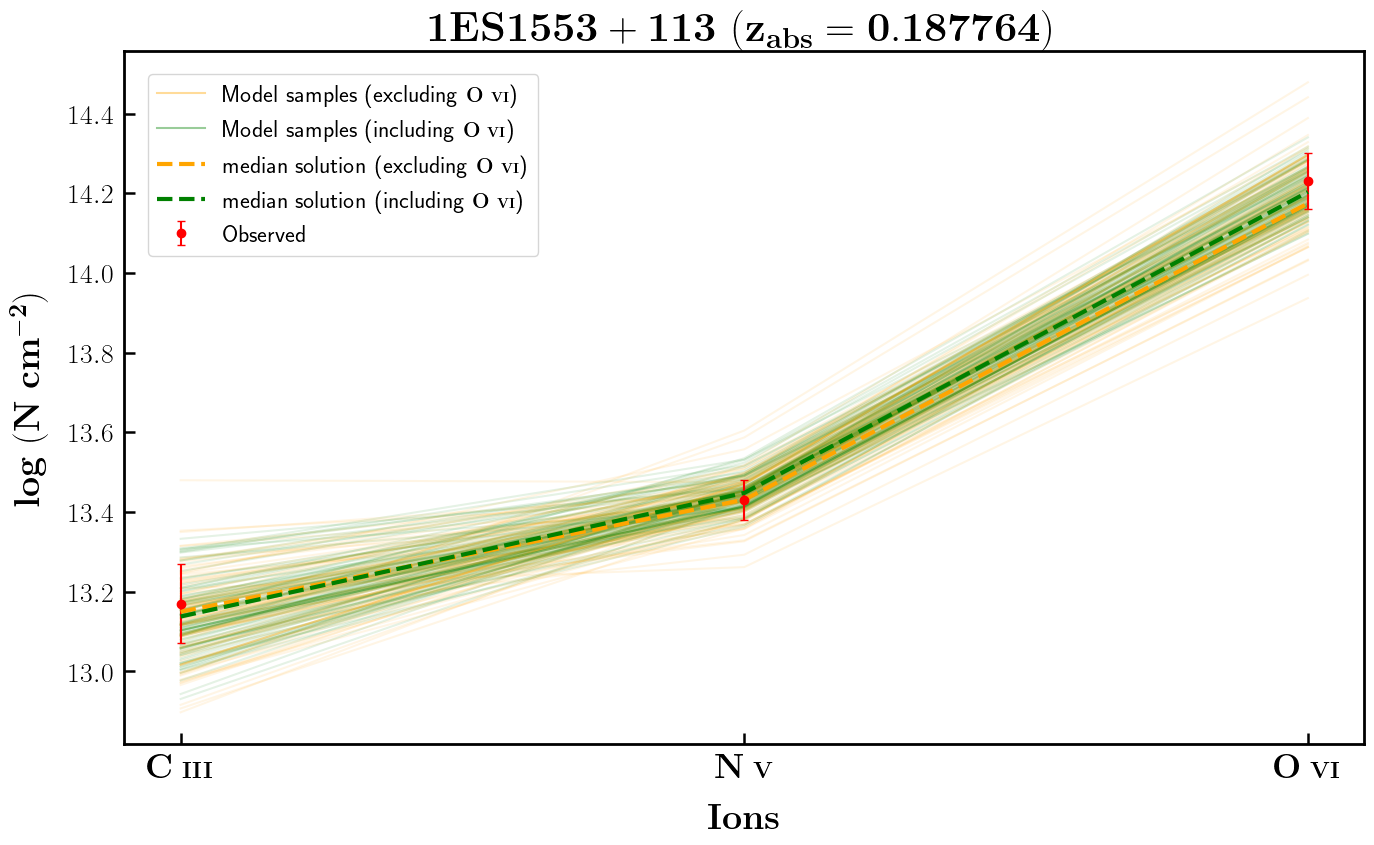
\includegraphics[width=10cm]{Figures/1es1553-z=0.187764-compI.png}
    \vspace*{-1mm}
    \caption{log N(\ion{H}{i}) [cm$^{-2}$]=12.76}
\end{figure}  

\end{frame}


\begin{frame}[noframenumbering]{\textbf{Ex : Uncertain}}

    \begin{figure}[!htbp]
    \centering
    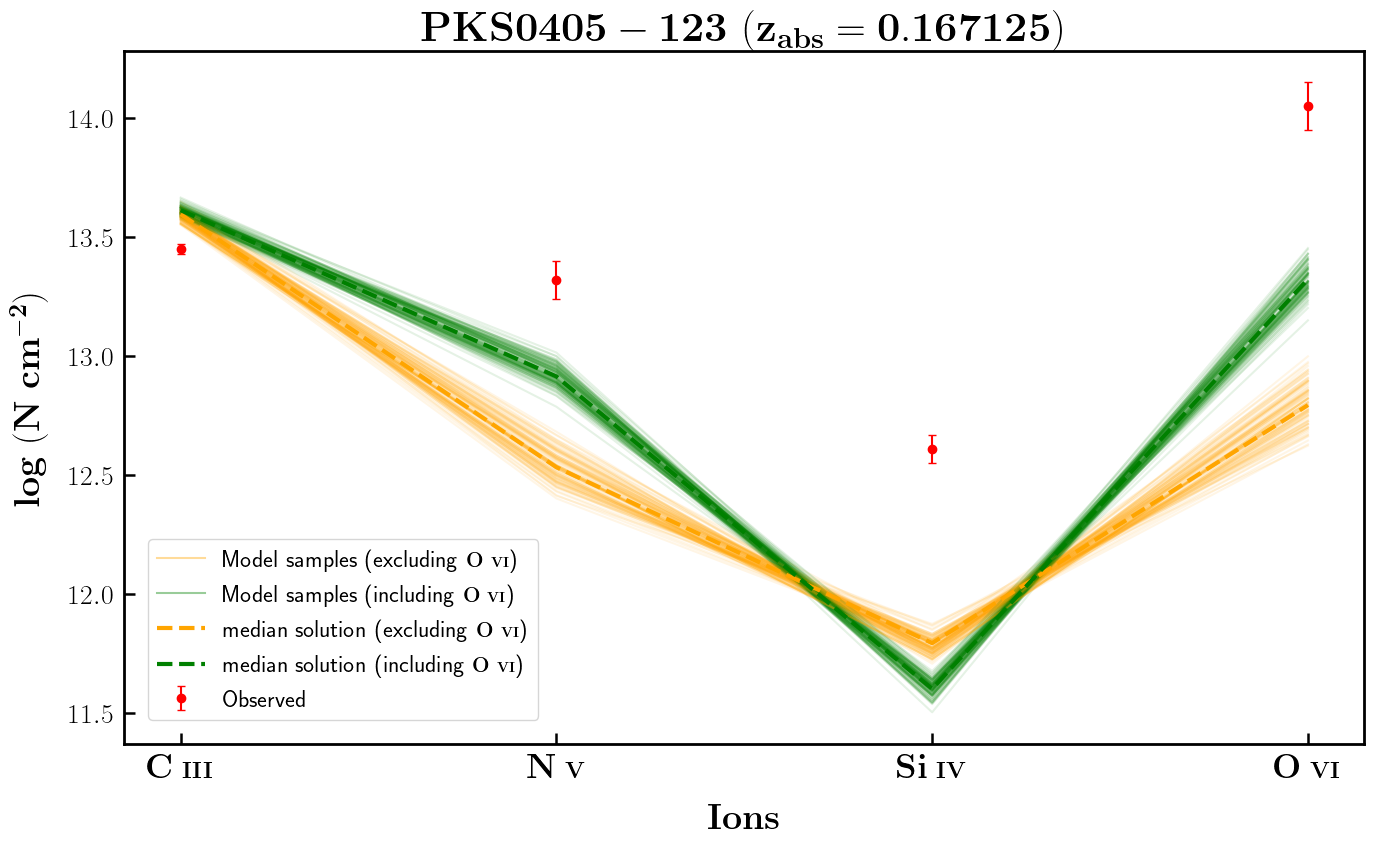
\includegraphics[width=10cm]{Figures/pks0405-z=0.167125-compII.png}
    \vspace*{-1mm}
    \caption{log N(\ion{H}{i}) [cm$^{-2}$]=13.46}
    \end{figure}  
    
    \end{frame}
